\chapter{Structured data}
\label{chap:data}
\glsresetall

\chapterprecishere{%
  Like families, tidy datasets are all alike, but every messy \\dataset is messy in its own way.
  \par\raggedleft--- \textup{Hadley Wickham}, Tidy Data}

As one expects, when we measure a phenomenon, the resulting data come in many different
formats.  For example, we can measure the temperature of a room using a thermometer.  The
resulting data is a number.  We can assess English proficiency using an essay test.  The
resulting data is a text.  We can register relationships between proteins and their
functions.  The resulting data is a graph.  Thus, it is important to understand the nature
of the data we are working with.

The most common data format is the \emph{structured data}.  Structured data refers to
information that is organized in a tabular format.
We restrict the kind of information we store in each cell, i.e. the data type of each
measurement.  The data type restrict the operations we can
perform on the data.  For example, we can perform arithmetic operations on numbers, but
not on text.  All cells in the same column must share the same data type.

In this chapter, I discuss the most common data types and the most common data formats.
More specifically, we are interested in how the semantics of the data are encoded in the
data format.  Database normalization and tidy data are two concepts that are very important
for the understanding of structured data.

As a result, the reader will be equipped with the mindset to perform data tasks
--- collection, integration, tidying, and exploration --- well.

\begin{mainbox}{Chapter remarks}

  \boxsubtitle{Contents}

  \startcontents[chapters]
  \printcontents[chapters]{}{1}{}
  \vspace{1em}

  \boxsubtitle{Context}

  \begin{itemize}
    \itemsep0em
    \item Data comes in many different formats.
    \item Good data analysis requires understanding the data types and their meaning.
  \end{itemize}

  \boxsubtitle{Objectives}

  \begin{itemize}
    \itemsep0em
    \item Understand the most common data types and formats.
    \item Enable the reader to perform data tasks well by associating data format and semantics.
  \end{itemize}

  \boxsubtitle{Takeaways}

  \begin{itemize}
    \itemsep0em
    \item The choice of the observational unit is not always straightforward.
    \item Format and types must reflect the information the solution will ``see'' in
      production.
  \end{itemize}
\end{mainbox}

{}
\clearpage

\section{Data types}

The most common classification of data types is Stevens' types: nominal, ordinal,
interval, and ratio.  Nominal data are data that can be classified into categories.
Ordinal data are data that can be classified into categories and ordered.  Interval data
are data that can be classified into categories, ordered, and measured in fixed units.
Ratio data are data that can be classified into categories, ordered, measured in fixed
units, and have a true zero.  In practice, they differ on the logical and arithmetic operations
we can perform on them.

\begin{tablebox}[label=tab:stevens]{Stevens' types.}
  \centering
  \rowcolors{2}{black!10!white}{}
  \begin{tabular}{cc}
    \toprule
    \textbf{Data type} & \textbf{Operations} \\
    \midrule
    Nominal & $=$ \\
    Ordinal & $=, <$ \\
    Interval & $=, <, +, - $ \\
    Ratio & $=, <, +, -, \times, \div$ \\
    \bottomrule
  \end{tabular}
  \tcblower
  Stevens' types are a classification of data types based on the operations we can perform
  on them.
\end{tablebox}

\Cref{tab:stevens} summarizes the allowed operations for each of Stevens' type.  All types
enable equality comparison.  Ordinal data can also be tested in terms of their order, but
they do not allow quantitative difference.  Interval data, on the other hand, allow
addition and subtraction.  Finally, the true zero of ratio data enable us to calculate
relative differences (multiplication and division).

For example, color are nominal data.  We can classify colors into categories, but we cannot
order them.  A categorical variable that classifies sizes in small, medium, and large is
ordinal data.  We can order the sizes, but we cannot say that the difference between small
and medium is the same as the difference between medium and large.  Temperature in Celsius
is interval data.  We can order temperatures, and we can say that the difference between
10 and 20 degrees is the same as the difference between 20 and 30 degrees.  However, we
cannot say that 20 degrees is twice as hot as 10 degrees.  Finally, weight is ratio data.
We can order weights, we can say that the difference between 10 and 20 kilograms is the
same as the difference between 20 and 30 kilograms, and we can say that 20 kilograms is
twice as heavy as 10 kilograms.

Nonetheless, Stevens' types do not exhaust all possibilities for data types.  For example,
probabilities are bounded at both ends, and thus do not tolerate arbitrary scale shifts.
\textcite{Paul1993}\footfullcite{Paul1993} provide interesting insights about data types.  Although I do not
agree with all his points, I think it is a good reading.  In particular, I agree with
his criticism of statements that data types are evident from the data independent of the
questions asked.  The same data can be interpreted in different ways depending on the
context and the goals of the analysis.

However, I do not agree with the idea that good data analysis does not assume data types.
I think that data scientists should be aware of the data types they are working with and
how they affect the analysis.  With no bias, there is no learning.  There is no such a
thing as a ``bias-free'' analysis, the amount of possible combinations of assumptions
easily grows out of control.  The data scientist must take responsibility for the
consequences of their assumptions.  Good assumptions and hypotheses are a key part of the
data science methodology.

When we work with structured data, two concepts are very important: database normalization
and tidy data.  Database normalization is mainly focused on the data storage.  Tidy data is
mainly focused on the requirements of data for analysis.  Both concepts have their
mathematical/logical foundations and tools for data handling.

\section{Database normalization}
\label{sec:normalization}

Database normalization is the process of organizing the columns and tables of a relational
database to minimize data redundancy and improve data integrity.  The need for database
normalization comes from the fact that the same data can be stored in many different ways.

Normal form is a state of a database that is free of certain types of data redundancy.
Before studying normal forms, we need to understand basic concepts in the database theory
and the basic operations in relational algebra.

\subsection{Relational algebra}

Relational algebra is a theory that uses algebraic structures to manipulate relations.
Consider the following concepts.

\paragraph{Relation}  A relation is a table with rows and columns that represent
an entity.  Each row, or tuple, is assumed to appear only once in the relation.  Each
column, or attribute, is assumed to have a unique name.

\paragraph{Projection}  The projection of a relation is the operation that returns a
relation with only the columns specified in the projection.  For example, if we have a
relation $X[A, B, C]$ and we perform the projection $\pi_{A, C}(X)$, we get a
relation with only the columns $A$ and $C$, i.e. $X[A, C]$.  The number of rows
in the resulting relation might be less than the number of rows in the original relation
because of repeated rows.

\paragraph{Join}  The (natural) join of two relations is the operation that returns a
relation with the columns of both relations.  For example, if we have two relations $S[U
\cup V]$ and $T[U \cup W]$, where $U$ is the common set of attributes, join $S \bowtie T$
of $S$ and $T$ is the relation with tuples $(u, v, w)$ such that $(u, v) \in S$ and $(u,
w) \in T$.  The generalized join is built up out of binary joins:  $\bowtie \left\{ R_1,
R_2, \dots, R_n \right\} = R_1 \bowtie R_2 \bowtie \dots \bowtie R_n$. Since the join
operation is associative and commutative, we can parenthesize however we want.

\paragraph{Functional dependency}  A functional dependency is a constraint between two
sets of attributes in a relation.  It is a statement that if two tuples agree on certain
attributes, then they must agree on another attribute.  Specifically, the \emph{functional
dependency} $U \to V$ holds in $R$ if and only if for every pair of tuples $t_1$ and $t_2$
in $R$ such that $t_1[U] = t_2[U]$, it is also true that $t_1[V] = t_2[V]$.

\paragraph{Multi-valued dependency}  A multi-valued dependency constrains
two sets of attributes in a relation.  The
\emph{multi-valued dependency} $U \twoheadrightarrow V$ holds in $R$ if and only if $R =
R[UV] \bowtie R[UW]$, where $W$ are the remaining attributes.  Note, however, that unlike
functional dependencies, multi-valued dependencies are not simple to interpret, so we
restrict our discussion to its mathematical properties\footnote{In fact, one might
naively think that a multi-valued dependency is a functional dependency between
many attributes.  However, this is not the case.}.

\paragraph{Join dependency}  A join dependency is a constraint between subsets of
attributes (not necessarily disjoint) in a relation.  $R$ obeys the join dependency $*
\left\{ X_1, X_2, \dots, X_n \right\}$ if $R = {\bowtie \left\{ R[X_1], R[X_2], \dots,
R[X_n] \right\}}$.

\subsection{Normal forms}

The normal forms are a series of progressive conditions that a relation must satisfy to
be considered normalized.  The normal forms are cumulative, i.e. a relation that is in
$n$-th normal form is also in $(n-1)$-th normal form.  The normal forms are a way to
reduce redundancy and improve data integrity.

\paragraph{First normal form (1NF)}  A relation is in 1NF if and only if all attributes
are atomic.  An attribute is atomic if it is not a set of attributes.  For example, the
relation $R[A, B, C]$ is in 1NF if and only if $A$, $B$, and $C$ are atomic.

\paragraph{Second normal form (2NF)}  A relation is in 2NF if and only if it is in 1NF
and every non-prime attribute is fully functionally dependent on the primary key.  A
non-prime attribute is an attribute that is not part of the primary key.  A primary key
is a set of attributes that uniquely identifies a tuple.  A non-prime attribute is fully
functionally dependent on the primary key if it is functionally dependent on the primary
key and not on any subset of the primary key.  For example, the relation $R[U \cup V]$ is
in 2NF if and only if $U \to X,~\forall X \in V$ and there is no $W \subset U$ such that
$W \to X,~\forall X \in V$.

\paragraph{Third normal form (3NF)}  A relation is in 3NF if and only if it is in 2NF
and every non-prime attribute is non-transitively dependent on the primary key.  A
non-prime attribute is non-transitively dependent on the primary key if it is not
functionally dependent on another non-prime attribute.  For example, the relation $R[U
\cup V]$ is in 3NF if and only if $U$ is the primary key and there is no $X \in V$ such
that $X \to Y,~\forall Y \in V$.

\paragraph{Boyce-Codd normal form (BCNF)}  A relation $R$ with attributes $X$ is in BCNF
if and only if it is in 2NF and for each nontrivial functional dependency $U \to V$ in
$R$, the functional dependency $U \to X$ is in $R$.  In other words, a relation is in BCNF
if and only if every functional dependency is the result of keys.

\paragraph{Fourth normal form (4NF)}  A relation $R$ with attributes $X$ is in 4NF if
and only if it is in 2NF and for each nontrivial multi-valued dependency $U \twoheadrightarrow
V$ in $R$, the functional dependency $U \to X$ is in $R$.  In other words, a relation is
in 4NF if and only if every multi-valued dependency is the result of keys.

\paragraph{Projection join normal form (PJNF)} A relation $R$ with attributes $X$ is in
PJNF\footnote{Also known as fifth normal form (5NF).  The authors themselves prefer
the term PJNF because it emphasizes to which operations the normal form applies.}
if and only if it is in 2NF and
the set of key dependencies\footnote{Key dependency is a functional dependency in the form
$K \to X$, where $X$ emcompasses all attributes of the relation.} of $R$ implies each join
dependency of $R$.  The PJNF guarantees that the
table cannot be decomposed without losing information (except by decompositions based on
keys).

The idea behind the definition of BCNF and 4NF are slightly different from the
PJNF.  In fact, if we consider that for each key dependency implies a join dependency, the
relation is in the so-called overstrong projection-join normal
form\footfullcite{Fagin1979}.  Such a level of normalization does not improve data storage
or eliminate inconsistencies.  In practice, it means that if a relation is in PJNF,
careless joins --- i.e. those that violate a join dependency --- produce
inconsistent results.

\paragraph{Simple example}  Consider the 2NF relation $R[A, B, C, D]$ with functional
dependencies $A \to B,~B \to C,~C \to D$.  The relation is not in 3NF because $C$ is
transitively dependent on $A$.  To normalize it, we can decompose it into the
relations $R_1[A, B, C]$ and $R_2[C, D]$.  Now, $R_2$ is in 3NF and $R_1$ is in 2NF, but
not in 3NF.  We can decompose $R_1$ into the relations $R_3[A, B]$ and $R_4[B, C]$.
The original relation can be reconstructed by $\bowtie \left\{ R_2, R_3, R_4 \right\}$.

\paragraph{Illustrative example of data integrity}  Consider a relation of students and
their grades.  The relation contains the attributes ``student'', ``course'', ``course
credits'', and ``grade''.  The primary key is the composite of ``student'' and ``course''.
The functional dependencies are ``student'' and ``course'' determine ``grade'', and
``course'' determines ``course credits''.  The relation is in 2NF but not 3NF.

\begin{tablebox}[label=tab:student-grade-illustration]{Student grade relation.}
  \centering
  \rowcolors{2}{black!10!white}{}
  \begin{tabular}{cccc}
    \toprule
    \textbf{Student} & \textbf{Course} & \textbf{Course credits} & \textbf{Grade} \\
    \midrule
    Alice & Math & 4 & A \\
    Alice & Physics & 3 & B \\
    Bob & Math & 4 & B \\
    Bob & Physics & 3 & A \\
    \bottomrule
  \end{tabular}
  \tcblower
  An example of a relation of students and their grades in 2NF.
\end{tablebox}

\Cref{tab:student-grade-illustration} shows an example of possible values of the relation.
If we decide to change the course credits of the course ``Math'' to 5, we must update the
two rows, otherwise the relation will be inconsistent.  A 3NF relation (see
\cref{tab:student-grade-illustration2}) would have the attributes ``course'' and ``course
credits'' in a separate relation, avoiding the possibility of data inconsistency.  If
needed, the relation would be reconstructed by a join operation.

\begin{tablebox}[label=tab:student-grade-illustration2]{Student grade relation in 3NF.}
  \centering
  \rowcolors{2}{black!10!white}{}
  \begin{tabular}{cc}
    \toprule
    \textbf{Course} & \textbf{Course credits} \\
    \midrule
    Math & 4 \\
    Physics & 3 \\
    \bottomrule
  \end{tabular}
  \quad
  \rowcolors{2}{black!10!white}{}
  \begin{tabular}{ccc}
    \toprule
    \textbf{Student} & \textbf{Course} & \textbf{Grade} \\
    \midrule
    Alice & Math & A \\
    Alice & Physics & B \\
    Bob & Math & B \\
    Bob & Physics & A \\
    \bottomrule
  \end{tabular}
  \tcblower
  An example of a relation of students and their grades in 3NF.
\end{tablebox}

\paragraph{Invalid join example} Consider the 2NF relation $R[ABC]$\footnote{Here we abreviate ${A,
B, C}$ as $ABC$.} such that the primary key is the composite of $A$, $B$, and $C$.  The
relation is thus in the 4NF, as no column is a determinant of another column.  Suppose,
however, the following constraint: if $(a, b, c')$, $(a, b', c)$, and $(a', b, c)$ are in
$R$, then $(a, b, c)$ is also in $R$.  This can be illustrated if we consider $A$ as a
agent, $B$ as a product, and $C$ as a company.  If an agent $a$ represents companies $c$ and
$c'$, and product $b$ is in his portfolio, then assuming both companies make $b$, $a$
must offer $b$ from both companies.

The relation is not in PJNF, as the join dependency $* \left\{ AB, AC, BC \right\}$ is not
implied by the primary key.  (In fact, the only functional dependency is the trivial $ABC
\to ABC$.)  In this case, to avoid redundancies and inconsistencies, we must split the
relation into the relations $R_1[AB]$, $R_2[AC]$, and $R_3[BC]$.

It is interesting to notice that in this case, the relation $R_1 \bowtie R_2$ might
contain tuples that do not make sense in the context of the original relation.  For
example, if $R_1$ contains $(a, b)$ and $R_2$ contains $(a, c')$, the join contains
$(a, b, c')$, which might not be a valid tuple in the original relation if $(b, c')$ is
not in $R_3$.

\begin{hlbox}{Important note on PJNF}
  \em
  This is very important to notice, as it is a common mistake to assume
  that the join of the decomposed relations always contains valid tuples.
\end{hlbox}

\paragraph{Valid joins example}  Consider the 2NF relation $R[A, B, C, D, E]$ with the functional
dependencies $A \to D$, $AB \to C$, and $B \to E$.  To make it PJNF, we can decompose it
into the relations $R_1[A, D]$, $R_2[A, B, C]$, and $R_3[B, E]$.  The original relation can
be reconstructed by $\bowtie \left\{ R_1, R_2, R_3 \right\}$.  However, unlike the
previous example, the join of the decomposed relations always contains valid tuples
--- excluding degenerate joins, where there are no common attributes.
The reason is that all join dependencies implied by the key dependencies are trivial when
reduced\footnote{I am investigating a formal proof based on \fullcite{Vincent1997}.}.

\section{Tidy data}

It is estimated that 80\% of the time spent on data analysis is spent on data preparation.
Usually, the same process is repeated many times in different datasets. The ideia is that
organized data carries the meaning of the data, reducing the time spent on handling
the data to get it into the right format for analysis.

Tidy data, proposed by \textcite{Wickham2014}\footfullcite{Wickham2014},
is a data format that provides a standardized way to organize data values within
a dataset.  The main advantage of tidy data is that it provides clear semantics with focus
on only one view of the data.

Many data formats might be ideal for particular tasks, such as raw data, dense tensors, or
normalized databases.  However, most of the statistical and machine learning methods
require a particular data format.  Tidy data is a data format that is appropriate to those
tasks.

% \begin{hlbox}{Wickham's thoughts on tidy data}
%   \em
%   Like families, tidy datasets are all alike but every messy dataset is messy in its own
%   way.
% \end{hlbox}

In an unrestricted table, the meaning of rows and columns are not fixed.  In a tidy table,
the meaning of rows and columns are fixed.  The semantics is more restrictive than usually
required for general tabular data.

\begin{tablebox}[label=tab:simple-messy]{Example of same data in different formats.}
  \centering
  \rowcolors{2}{black!10!white}{}
  \begin{tabular}{ccc}
    \toprule
     & \textbf{Cases (2019)} & \textbf{Cases (2020)} \\
    \midrule
    \textbf{Brazil} & 100 & 200 \\
    \textbf{USA} & & 400 \\
    \bottomrule
  \end{tabular}
  \\[1em]
  \begin{tabular}{ccc}
    \toprule
    & \textbf{Brazil} & \textbf{USA} \\
    \midrule
    \textbf{Cases (2019)} & 100 & \\
    \textbf{Cases (2020)} & 200 & 400 \\
    \bottomrule
  \end{tabular}
  \tcblower
  The same data in different formats.  Both are considered messy by Wickham.
\end{tablebox}

\Cref{tab:simple-messy} shows an example of the same data in different formats.  Although
they emphasize different aspects (especially for visualization) of the data, both contain
the same amount of information.  They are considered messy by Wickham because the meaning
of the rows and columns are not fixed.

It is based on the idea that a dataset is a collection of values, where:
\begin{itemize}
  \itemsep0em
  \item Each \emph{value} belongs to a variable and an observation.
  \item Each \emph{variable}, represented by a column, contains all values that measure
    the same attribute across (observational) units.
  \item Each \emph{observation}, represented by a row, contains all values measured on the
    same unit across attributes.
  \item \emph{Attributes} are the characteristics of the units, e.g. height, temperature,
    duration.
  \item \emph{Observational units} are the individual entities being measured, for
    instance, a person, a day, an experiment.
\end{itemize}
Table \ref{tab:tidy} summarizes the main concepts.

\begin{tablebox}[label=tab:tidy]{Tidy data concepts.}
  \centering
  \rowcolors{2}{black!10!white}{}
  \begin{tabular}{cccc}
    \toprule
    \textbf{Concept} & \textbf{Structure} & \textbf{Contains} & \textbf{Across} \\
    \midrule
    Variable & Column & Same attribute & Units \\
    Observation & Row & Same unit & Attributes \\
    \bottomrule
  \end{tabular}
\end{tablebox}

\begin{tablebox}[label=tab:simple-tidy]{Example of tidy data.}
  \centering
  \rowcolors{2}{black!10!white}{}
  \begin{tabular}{ccc}
    \toprule
    \textbf{Country} & \textbf{Year} & \textbf{Cases} \\
    \midrule
    Brazil & 2019 & 100 \\
    Brazil & 2020 & 200 \\
    USA & 2019 & \\
    USA & 2020 & 400 \\
    \bottomrule
  \end{tabular}
  \tcblower
  An example of tidy data from the data in \cref{tab:simple-messy}.
\end{tablebox}

If we follow this structure, the meaning of data is implicit in the table itself.
\Cref{tab:simple-tidy} shows the same data in a tidy format.  The table is now longer, but
the variables and observations are clear from the table itself.

However, it is not always trivial to organize data in a tidy format.  Usually, we have
more than one level of observational units, each one represented by a table.  Moreover,
there might exist more than one way to define what are the observational units in a
dataset\footnote{Although, Wickham himself implies that there is only one possible way to
define the observational units of the dataset.}.

To organize data in a tidy format, one can consider that:
\begin{itemize}
  \itemsep0em
  \item Attributes are functionally related among themselves --- e.g. Z is a linear
    combination of X and Y, or X and Y are correlated, or $P(X, Y)$ follows some joint distribution.
  \item Units can be grouped or compared --- e.g. person A is taller than person B, or
    the temperature in day 1 is higher than in day 2.
\end{itemize}

A particular point that tidy data do not address is that values in a column might not be
in the same scale or unit of measurement\footnote{Observational unit is not the same
concept as unit of measurement.}.  For example, a column might contain the
temperature in an experiment, and another column might contain the unit of measurement
that was used to measure the temperature.  This is a common problem in databases, and it
must be addressed for machine learning and statistical methods to work properly.

Note that the order of the rows and columns is not important.  However, it might be
convenient to sort data in a particular way to facilitate the understanding.  For
instance, one usually expects that the first columns are \emph{fixed
variables}\footnote{Closely related (and potentially the same as) key in database
theory.} --- i.e. variables that are not the result of a measurement but that describe the
experimental design ---, and the last columns
are \emph{measured variables}.  Also, arranging rows by some variable might highlight some
pattern in the data.

Usually, columns are named --- the collection of all column names is called the
header, while rows are usually numerically indexed.

\subsection{Common messy datasets}
\label{sub:messy}

\textcite{Wickham2014}\footfullcite{Wickham2014} lists some common problems with messy
datasets and how to tidy them.  In this subsection, we focus on the problems and the
tidy solutions.  The data handling operations that enables us to tidy the data are
presented in \cref{chap:handling}.  Readers interested in a step by step guide for data
tidying are encouraged to read \textcite{Wickham2023}\footfullcite{Wickham2023}.

The problems are summarized below.

\clearpage
\subsubsection{Headers are values, not variable names}  For example, consider
\cref{tab:messy1}.  This table is not tidy because the column headers are values, not
variable names.  This format is frequently used in presentations since it is more compact.
It is also useful to perform matrix operations. However, it is not appropriate for general
analysis.

\begin{tablebox}[label=tab:messy1]{Messy table, from Pew Forum dataset, where headers are values, not variable names.}
  \centering
  \rowcolors{2}{black!10!white}{}
  \begin{tabular}{l r r r c}
    \toprule
    \textbf{Religion} & \textbf{<\$10k} & \textbf{\$10-20k} & \textbf{\$20-30k} & \textbf{\dots} \\
    \midrule
    Agnostic & 27 & 34 & 60 & \dots \\
    Atheist & 12 & 27 & 37 & \dots \\
    Buddhist & 27 & 21 & 30 & \dots \\
    \dots & \dots & \dots & \dots & \dots \\
    \bottomrule
  \end{tabular}
\end{tablebox}

To make it tidy, we can transform it into the \cref{tab:tidy1} by explicitly introducing
variables \emph{Income} and \emph{Frequency}.
Note that the table is now longer, but it is also narrower.  This is a common pattern when
fixing this kind of issue.  The table is now tidy because the column headers are variable
names, not values.

\begin{tablebox}[label=tab:tidy1]{Tidy version of \cref{tab:messy1} where values are correctly moved.}
  \centering
  \rowcolors{2}{black!10!white}{}
  \begin{tabular}{l l r}
    \toprule
    \textbf{Religion} & \textbf{Income} & \textbf{Frequency} \\
    \midrule
    Agnostic & <\$10k & 27 \\
    Agnostic & \$10-20k & 34 \\
    Agnostic & \$20-30k & 60 \\
    \dots & \dots & \dots \\
    Atheist & <\$10k & 12 \\
    Atheist & \$10-20k & 27 \\
    Atheist & \$20-30k & 37 \\
    \dots & \dots & \dots \\
    \bottomrule
  \end{tabular}
\end{tablebox}

\clearpage
\subsubsection{Multiple variables are stored in one column}  For example, consider the
\cref{tab:messy2}.  This table is not tidy because the column --- interestly called
\emph{column} ---, contains multiple variables.  This format is frequent, and sometimes the
column name contains the names of the variables.  Sometimes it is very hard to separate
the variables.

\begin{tablebox}[label=tab:messy2]{Messy table, from TB dataset, where multiple variables are stored in one column.}
  \centering
  \rowcolors{2}{black!10!white}{}
  \begin{tabular}{l l l r c}
    \toprule
    \textbf{country} & \textbf{year} & \textbf{column} & \textbf{cases} & \textbf{\dots} \\
    \midrule
    AD & 2000 & m014 & 0 & \dots \\
    AD & 2000 & m1524 & 0 & \dots \\
    AD & 2000 & m2534 & 1 & \dots \\
    AD & 2000 & m3544 & 0 & \dots \\
    \dots & \dots & \dots & \dots \\
    \bottomrule
  \end{tabular}
\end{tablebox}

To make it tidy, we can transform it into the \cref{tab:tidy2}.  Two columns are created
to contain the variables \emph{Sex} and \emph{Age}, and the old column is removed.  The
table keeps the same number of rows, but it is now wider.  This is a common pattern when
fixing this kind of issue.  The new version usually fixes the issue of correctly
calculating ratios and frequency.

\begin{tablebox}[label=tab:tidy2]{Tidy version of \cref{tab:messy2} where values are correctly moved.}
  \centering
  \rowcolors{2}{black!10!white}{}
  \begin{tabular}{l l l l r c}
    \toprule
    \textbf{country} & \textbf{year} & \textbf{sex} & \textbf{age} & \textbf{cases} & \textbf{\dots} \\
    \midrule
    AD & 2000 & m & 0--14 & 0 & \dots \\
    AD & 2000 & m & 15--24 & 0 & \dots \\
    AD & 2000 & m & 25--34 & 1 & \dots \\
    AD & 2000 & m & 35--44 & 0 & \dots \\
    \dots & \dots & \dots & \dots & \dots \\
    \bottomrule
  \end{tabular}
\end{tablebox}

\clearpage
\subsubsection{Variables are stored in both rows and columns}  For example, consider the
\cref{tab:messy3}.  This is the most complicated case of messy data.  Usually, one of the
columns contains the names of the variables, in this case the column \emph{element}.

\begin{tablebox}[label=tab:messy3]{Messy table, adapted from airquality dataset, where variables are stored in both rows and columns.}
  \centering
  \rowcolors{2}{black!10!white}{}
  \begin{tabular}{llllcccc}
    \toprule
    \textbf{id} & \textbf{year} & \textbf{mo.} & \textbf{element} & \textbf{d1} & \textbf{d2} & \textbf{\dots} & \textbf{d31} \\
    \midrule
    MX17004 & 2010 & 1 & tmax &    & 24 & \dots & 27 \\
    MX17004 & 2010 & 1 & tmin & 14 &    & \dots &    \\
    MX17004 & 2010 & 2 & tmax & 27 & 24 & \dots & 27 \\
    MX17004 & 2010 & 2 & tmin & 14 &    & \dots & 13 \\
    \dots & \dots & \dots & \dots & \dots & \dots & \dots & \dots \\
    \bottomrule
  \end{tabular}
\end{tablebox}

To fix this issue, we must first decide which column contains the names of the variables.
Then, we must lengthen the table in function of the variables (and potentially their
names), as seen in \cref{tab:tidy3a}.

\begin{tablebox}[label=tab:tidy3a]{Partial solution to tidy \cref{tab:messy3}. Note that
  the table is now longer.}
  \centering
  \rowcolors{2}{black!10!white}{}
  \begin{tabular}{lllc}
    \toprule
    \textbf{id} & \textbf{date} & \textbf{element} & \textbf{value} \\
    \midrule
    MX17004 & 2010-01-01 & tmax &    \\
    MX17004 & 2010-01-01 & tmin & 14 \\
    MX17004 & 2010-01-02 & tmax & 24 \\
    MX17004 & 2010-01-02 & tmin &    \\
    \dots & \dots & \dots & \dots \\
    \bottomrule
  \end{tabular}
\end{tablebox}

\clearpage
Afterwards, we widen the table in function of their names.  Finally, we remove
implicit information, as seen in \cref{tab:tidy3b}.

\begin{tablebox}[label=tab:tidy3b]{Tidy version of \cref{tab:messy3} where values are correctly moved.}
  \centering
  \rowcolors{2}{black!10!white}{}
  \begin{tabular}{llcc}
    \toprule
    \textbf{id} & \textbf{date} & \textbf{tmin} & \textbf{tmax} \\
    \midrule
    MX17004 & 2010-01-01 & 14 &    \\
    MX17004 & 2010-01-02 &    & 24 \\
    \dots & \dots & \dots & \dots \\
    \bottomrule
  \end{tabular}
\end{tablebox}

\subsubsection{Multiple types of observational units are stored in the same table}  For
example, consider the \cref{tab:messy4}.  It is very common during data collection that
many observational units are registered in the same table.

\begin{tablebox}[label=tab:messy4]{Messy table, adapted from billboard dataset, where multiple types of observational units are stored in the same table.}
  \centering
  \rowcolors{2}{black!10!white}{}
  \begin{tabular}{lllll}
    \toprule
    \textbf{year} & \textbf{artist} & \textbf{track} & \textbf{date} & \textbf{rank} \\
    \midrule
    2000 & 2 Pac & Baby Don't Cry & 2000-02-26 & 87 \\
    2000 & 2 Pac & Baby Don't Cry & 2000-03-04 & 82 \\
    2000 & 2 Pac & Baby Don't Cry & 2000-03-11 & 72 \\
    2000 & 2 Pac & Baby Don't Cry & 2000-03-18 & 77 \\
    \dots & \dots & \dots & \dots & \dots \\
    2000 & 2Ge+her & The Hardest\dots & 2000-09-02 & 91 \\
    2000 & 2Ge+her & The Hardest\dots & 2000-09-09 & 87 \\
    2000 & 2Ge+her & The Hardest\dots & 2000-09-16 & 92 \\
    \dots & \dots & \dots & \dots & \dots \\
    \bottomrule
  \end{tabular}
\end{tablebox}

To fix this issue, we must each observation unit must be moved to a different table.
Sometimes, it is useful to create unique identifiers for each observation.
The separation avoids several types of potential inconsistencies.  However, take into
account that during data analysis, it is possible that we have to denormalize them.  The
two resulting tables are shown in \cref{tab:tidy4a} and \cref{tab:tidy4b}.

\begin{tablebox}[label=tab:tidy4a]{Tidy version of \cref{tab:messy4} containing the observational unit \emph{track}.}
  \centering
  \rowcolors{2}{black!10!white}{}
  \begin{tabular}{lll}
    \toprule
    \textbf{track id} & \textbf{artist} & \textbf{track} \\
    \midrule
    1 & 2 Pac & Baby Don't Cry \\
    2 & 2Ge+her & The Hardest Part Of Breaking Up \\
    \dots & \dots & \dots \\
    \bottomrule
  \end{tabular}
\end{tablebox}

\begin{tablebox}[label=tab:tidy4b]{Tidy version of \cref{tab:messy4} containing the observational unit \emph{rank of the track in certain week}.}
  \centering
  \rowcolors{2}{black!10!white}{}
  \begin{tabular}{lll}
    \toprule
    \textbf{track id} & \textbf{date} & \textbf{rank} \\
    \midrule
    1 & 2000-02-26 & 87 \\
    1 & 2000-03-04 & 82 \\
    1 & 2000-03-11 & 72 \\
    1 & 2000-03-18 & 77 \\
    \dots & \dots & \dots \\
    2 & 2000-09-02 & 91 \\
    2 & 2000-09-09 & 87 \\
    2 & 2000-09-16 & 92 \\
    \dots & \dots & \dots \\
    \bottomrule
  \end{tabular}
\end{tablebox}

\subsubsection{A single observational unit is stored in multiple tables}  For example, consider
\cref{tab:messy5a,tab:messy5b}.  It is very common during data
collection that a single observational unit is stored in multiple tables.  Usually, the
table (or file) itself represents the value of a variable.  When columns are compatible,
it is straightforward to combine the tables.

\begin{tablebox}[label=tab:messy5a]{Messy tables, adapted from nycflights13 dataset, where
  a single observational unit is stored in multiple tables.  Assume that the origin
  filename is called \texttt{2013.csv}.}
  \centering
  \rowcolors{2}{black!10!white}{}
  \begin{tabular}{llll}
    \toprule
    \textbf{month} & \textbf{day} & \textbf{time} & \textbf{\dots} \\
    \midrule
    1 & 1 & 517 & \dots \\
    1 & 1 & 533 & \dots \\
    1 & 1 & 542 & \dots \\
    1 & 1 & 544 & \dots \\
    \dots & \dots & \dots & \dots \\
    \bottomrule
  \end{tabular}
\end{tablebox}

\begin{tablebox}[label=tab:messy5b]{Messy tables, adapted from nycflights13 dataset, where
  a single observational unit is stored in multiple tables.  Assume that the origin
  filename is called \texttt{2014.csv}.}
  \centering
  \rowcolors{2}{black!10!white}{}
  \begin{tabular}{llll}
    \toprule
    \textbf{month} & \textbf{day} & \textbf{time} & \textbf{\dots} \\
    \midrule
    1 & 1 & 830 & \dots \\
    1 & 1 & 850 & \dots \\
    1 & 1 & 923 & \dots \\
    1 & 1 & 1004 & \dots \\
    \dots & \dots & \dots & \dots \\
    \bottomrule
  \end{tabular}
\end{tablebox}

To fix this issue, we must first make the columns compatible.  Then, we can combine the
tables adding a new column that identifies the origin of the data.  The resulting table is
shown in \cref{tab:tidy5}.

\begin{tablebox}[label=tab:tidy5]{Tidy data where \cref{tab:messy5a,tab:messy5b} are combined.}
  \centering
  \rowcolors{2}{black!10!white}{}
  \begin{tabular}{lllll}
    \toprule
    \textbf{year} & \textbf{month} & \textbf{day} & \textbf{time} & \textbf{\dots} \\
    \midrule
    2013 & 1 & 1 & 517 & \dots \\
    2013 & 1 & 1 & 533 & \dots \\
    2013 & 1 & 1 & 542 & \dots \\
    2013 & 1 & 1 & 544 & \dots \\
    \dots & \dots & \dots & \dots & \dots \\
    2014 & 1 & 1 & 830 & \dots \\
    2014 & 1 & 1 & 850 & \dots \\
    2014 & 1 & 1 & 923 & \dots \\
    2014 & 1 & 1 & 1004 & \dots \\
    \dots & \dots & \dots & \dots & \dots \\
    \bottomrule
  \end{tabular}
\end{tablebox}

\clearpage
\section{Bridging normalization, tidiness, and data theory}
\label{sub:bridge}

First and foremost, both concepts, normalization and tidy data, are not in conflict.

In data normalization, given a set of functional, multivalued and join dependencies, there
exists a normal form that is free of redundancy.  In tidy data,
\textcite{Wickham2023}\footfullcite{Wickham2023} also state that there is only one way to organize the given data.

\textcite{Wickham2014}\footfullcite{Wickham2014} state that tidy data is 3NF.  However, he does not provide a
formal proof.  Since tidy data focuses on data analysis and not on data storage, I argue
that there is more than one way to organize the data in a tidy format.  It actually
depends on what you define as the observational unit.

Moreover, both of them are related to the philosophical concept of substance (οὐσία) ---
see \cref{sub:phenomena}.
Entities and observational units are substances while attributes are predicates.
Each tuple or observation are primary substances, i.e. substances that contrasts with
everything else, particular, individual.

We can also understand primary keys and fixed variables as the same concept.  They both
describe the sample uniquely.  They connect the entities/observational
units to the remaining of the attributes.  They also should never be fed into a learning
machine (more details in \cref{chap:slt}), since they are individual and thus not
appropriate to generalize.

\begin{tablebox}[label=fig:bridge]{Terms in different contexts.}
  \centering
  \rowcolors{2}{black!10!white}{}
  \begin{tabular}{ccc}
    \toprule
    \textbf{Relations} & \textbf{Tidy data} & \textbf{Philosophy} \\
    \midrule
    Entities & Observational units & Substance \\
    Tuple & Observation & Primary substance \\
    %Attribute & Attribute & Predicate \\
    Primary key & Fixed variables & Univocal name \\
    Non-prime attr. & Measured variable & Predicate \\
    \bottomrule
  \end{tabular}
  \tcblower
  Equivalence (or similarity) of data-related terms in different contexts.
  The ontological understanding of the data influences the way it is organized.
\end{tablebox}

\Cref{fig:bridge} summarizes the equivalence (or similarity) of terms in different
contexts.

\subsection{Tidy or not tidy?}
\label{sub:tidy-not-tidy}

Consider the following example.  We want to study the \emph{phenomenon} temperature in a
certain city.  We fix three sensors in different locations to measure the temperature.  We
collect data three times a day.  If we consider as the observational unit the
event of measuring the temperature, we can organize the data in a tidy format as shown in
\cref{tab:temp1}.

\begin{tablebox}[label=tab:temp1]{Tidy data where the observational unit is the event of measuring the temperature.}
  \centering
  \rowcolors{2}{black!10!white}{}
  \begin{tabular}{lllc}
    \toprule
    \textbf{date} & \textbf{time} & \textbf{sensor} & \textbf{temperature} \\
    \midrule
    2023-01-01 & 00:00 & 1 & 20 \\
    2023-01-01 & 00:00 & 2 & 21 \\
    2023-01-01 & 00:00 & 3 & 22 \\
    2023-01-01 & 08:00 & 1 & 21 \\
    2023-01-01 & 08:00 & 2 & 22 \\
    2023-01-01 & 08:00 & 3 & 23 \\
    \dots & \dots & \dots & \dots \\
    \bottomrule
  \end{tabular}
\end{tablebox}

However, since the sensors are fixed, we can consider the observational unit as the
\emph{temperature at some time}.  In this case, we can organize the data in a tidy format
as shown in \cref{tab:temp2}.

\begin{tablebox}[label=tab:temp2]{Tidy data where the observational unit is the temperature at some time.}
  \centering
  \rowcolors{2}{black!10!white}{}
  \begin{tabular}{llccc}
    \toprule
    \textbf{date} & \textbf{time} & \textbf{temp. 1} & \textbf{temp. 2} & \textbf{temp. 3} \\
    \midrule
    2023-01-01 & 00:00 & 20 & 21 & 22 \\
    2023-01-01 & 08:00 & 21 & 22 & 23 \\
    \dots & \dots & \dots & \dots & \dots \\
    \bottomrule
  \end{tabular}
\end{tablebox}

In both cases, one can argue that the data is also normalized.  In the first case, the
primary key is the composite of the columns \emph{date}, \emph{time}, and \emph{sensor}.
In the second case, the primary key is the composite of the columns \emph{date} and
\emph{time}.

One can state that the first form is more appropriate, since it is flexible to add more
sensors or sensor-specific attributes (using an extra table).  However, the second form is very natural for machine learning and statistical
methods.  Given the definition of tidy data, I believe both forms are correct.  It is
just a matter of what ontological view you have of the data.

\begin{tablebox}[label=tab:body1]{Tidy data for measuments of a person body.}
  \centering
  \rowcolors{2}{black!10!white}{}
  \begin{tabular}{lccc}
    \toprule
    \textbf{name} & \textbf{chest} & \textbf{waist} & \textbf{hip} \\
    \midrule
    Alice & 90 & 70 & 100 \\
    Bob & 100 & 110 & 110 \\
    \dots & \dots & \dots & \dots \\
    \bottomrule
  \end{tabular}
\end{tablebox}

Still, one can still argue that the sensors share the same nature and thus only the first
form is correct (or can even insist that the more flexible form is the correct one).
Consider however the data in \cref{tab:body1}.  The observational unit is the person, and
the attributes are the body measurements.

\begin{tablebox}[label=tab:body2]{Another tidy data for measurements of a person body.}
  \centering
  \rowcolors{2}{black!10!white}{}
  \begin{tabular}{llc}
    \toprule
    \textbf{name} & \textbf{body part} & \textbf{measurement} \\
    \midrule
    Alice & chest & 90 \\
    Alice & waist & 70 \\
    Alice & hip & 100 \\
    Bob & chest & 100 \\
    Bob & waist & 110 \\
    Bob & hip & 110 \\
    \dots & \dots & \dots \\
    \bottomrule
  \end{tabular}
\end{tablebox}

If we apply the same logic of \cref{tab:temp1}, data in \cref{tab:body1} becomes
\cref{tab:body2}.  Now, the observational unit is the measurement of a body part of a
given person.  Now, we can easily include more body parts.  Let us say that we want to add
the head circumference.  We just need to include rows such as ``Alice, head, 50'' and
``Bob, head, 55''.  Moreoer, what if we want to add the height of the person? Should we
create another table (with ``name'' and ``height'') or should we consider ``height'' seen
as another body part (even though it seems weird to consider the full body a part of the
body)?

In the first version of the data (\cref{tab:temp1}), it would be trivial to include head
circumference and height.  In the second version, the choice becomes inconvenient.  This
table seems ``overtidy''.  If the first fits well for the analysis, it should be
preferred.

In summary, tidiness is a matter of perspective.

\subsection{Change of observational unit}
\label{sub:change-unit}

Another very interesting conjecture is whether we can formalize the eventual \emph{change
of observational unit} in terms of the order that joins and grouping operations are
performed.

Consider the following example: the relation $R[A, B, C, D, E]$ and the functional
dependencies $A \to D$, $B \to E$, and $AB \to C$.  The relation can be normalized up to
3NF by following one of the decomposition trees shown in \cref{fig:decomp}.
Every decomposition tree must take into account that the join of the projections are
lossless and dependency preserving.

\begin{figurebox}[label=fig:decomp]{Decomposition trees for the relation $R[ABCDE]$ and
  the functional dependencies $A \to D$, $B \to E$, and $AB \to C$ to reach 3NF.}
  \centering
  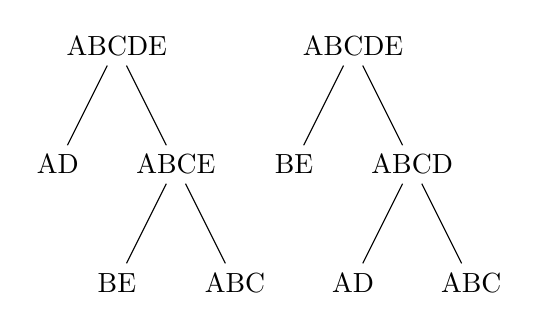
\begin{tikzpicture}
    \node (root1) at (0, 0) {ABCDE}
      child {node {AD}}
      child {node {ABCE}
        child {node {BE}}
        child {node {ABC}}};
    \node (root2) at (3, 0) {ABCDE}
      child {node {BE}}
      child {node {ABCD}
        child {node {AD}}
        child {node {ABC}}};
  \end{tikzpicture}
\end{figurebox}

Note that the decomposition that splits first $R[ABC]$ is not valid, since the resulting
relation $R[AB]$ is not a consequences of a functional dependency, see
\cref{fig:wrongdecomp}.

\begin{figurebox}[label=fig:wrongdecomp]{Invalid decomposition trees for the relation $R[ABCDE]$.}
  \centering
  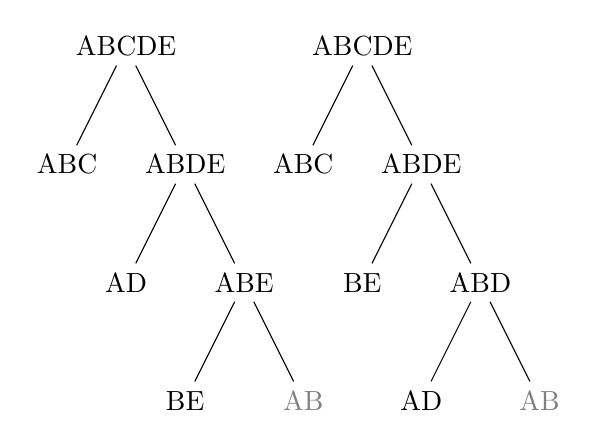
\begin{tikzpicture}
    \node (root1) at (0, 0) {ABCDE}
      child {node {ABC}}
      child {node {ABDE}
        child {node {AD}}
        child {node {ABE}
          child {node {BE}}
          child {node[gray] {AB}}}};
    \node (root2) at (3, 0) {ABCDE}
      child {node {ABC}}
      child {node {ABDE}
        child {node {BE}}
        child {node {ABD}
          child {node {AD}}
          child {node[gray] {AB}}}};
  \end{tikzpicture}
  \tcblower
  We consider the functional dependencies $A \to D$, $B \to E$, and $AB \to C$.
  Note that $R[AB]$ is not a consequence of a functional dependency.
\end{figurebox}

In this kind of relation schema, we have a set of key attributes, here $\mathcal{K} = AB$,
and a set of non-prime attributes, here $\mathcal{N} = CDE$.  Note that the case
$\mathcal{K} \cap \mathcal{N} = \emptyset$ is the simplest we can have.

Observe, however, that transitive dependencies\footnote{Actually, when an attribute is
both key and non-prime, some joins may generate invalid tables.} and complex join
dependencies restrict even further the joins we are allowed to perform.
% \textcolor{red}{Further formalization and study is under progress.}

Now, consider a very common case: in our dataset, keys are unknown.  Let $A$ be a student
id, $B$ be the course id, $D$ be the student age, $E$ be the course load, and $C$ be the
student grade at the course.  If only $CDE$ is known, the table $R[CDE]$ is already tidy
--- and the observational unit is the enrollment --- once there is no key to perform any
kind of normalization.  This happens in many cases where privacy is a concern.

\begin{tablebox}[label=tab:student]{Example of a dataset where the observational unit is the student.}
  \centering
  \rowcolors{2}{black!10!white}{}
  \begin{tabular}{llll}
    \toprule
    \textbf{A (student)} & \textbf{B (course)} & \textbf{C (grade)} & \textbf{E (load)} \\
    \midrule
    1 & 1 & 7 & 60 \\
    1 & 2 & 8 & 30 \\
    2 & 1 & 7 & 60 \\
    2 & 3 & 9 & 40 \\
    \dots & \dots & \dots & \dots \\
    \bottomrule
  \end{tabular}
  \\[1em]
  \begin{tabular}{lll}
    \toprule
    \textbf{A (student)} & \textbf{F (average grade)} & \textbf{G (total load)} \\
    \midrule
    1 & 7.5 & 90 \\
    2 & 8 & 100 \\
    \dots & \dots & \dots \\
    \bottomrule
  \end{tabular}
  \tcblower
  Relation $R[ABCE]$ becomes $R[AFG]$ after the summarization operation.  Now each row
  represents a student (values in $A$ are unique).
\end{tablebox}

But we can also consider that the observational unit is the student.  In this case, we
must perform joins traversing the leftmost decomposition tree in \cref{fig:decomp} from
bottom to top.  After each join, a summarization operation is performed on the relation
considering the student as the observational unit, i.e. over attribute $A$.  The first
join results in relation $R[ABCE]$ and the summarization operation results in a new
relation $R[AFG]$ where $F$ is the average grade and $G$ is the total course load taken by
the student (see \cref{tab:student}).  They all calculated based on the rows that are grouped in function of $A$.
It is important to notice that, after the summarization operation, all observations must
contain a different value of $A$.  The second join results in relation $R[ADFG] = R[AD]
\bowtie R[AFG]$.  This relation has functional dependency $A \to DFG$, and it is in 3NF
(which is also tidy).

Unfortunately, it is not trivial to calculate all possible decomposition trees for a given
dataset.  It is up to the data scientist to decide which directions to follow.  However,
it is important to notice that the order of the joins and summarization operations are
crucial to the final result.
%\textcolor{red}{Further formalization and study is under progress.}

\section{Data semantics and interpretation}

In the rest of the book, we focus on a statistical view of the data.  Besides the
functional dependencies, we also consider the statistical dependencies of data.  For
instance, attributes $A$ and $B$ might not be functionally dependent, but they might exits
unknown $P(A, B)$ that we can estimate from the data.  Each observed value of a key can
represent a instance of a random variable, and the other attributes can represent
measured attributes or calculated properties.

For data analysis, it is very important to understand the relationships between the
observations.  For example, we might want to know if the observations are independent, if
they are identically distributed, or if there is a known selection bias.  We might also
want to know if the observations are dependent on time, and if there are hidden variables
that affect the observations.

Following wrong assumptions can lead to wrong conclusions.  For example, if we assume that
the observations are independent, but they are not, we might underestimate the variance of
the estimators.

Although we do not focus on time series, we must consider the temporal dependence of the
observations.  For example, we might want to know how the observation $x_t$ is affected by
$x_{t-1}$, $x_{t-2}$, and so on.  We might also want to know if Markov property holds,
and if there is periodicity and seasonality in the data.

For the sake of the scope of this book, we suggest that any prediction on temporal data
should be done in the state space, where it is safer to assume that observations are
independent and identically distributed.  This is a common practice in reinforcement
learning and deep learning. Takens' theorem\footfullcite{Takens1980} allows you to
reconstruct the state space of a dynamical system using time-delay embedding. Given a
single observed time series, you can create a multidimensional representation of the
underlying dynamical system by embedding the time series in a higher-dimensional space.
This embedding can reveal the underlying dynamics and structure of the system.

\section{Unstructured data}

Unstructured data are data that do not have a predefined data model or are not organized
in a predefined manner.  For example, text, images, and videos are unstructured data.

Every unstructured dataset can be converted into a structured one.  However, the
conversion process is not always straightforward nor lossless.  For example, we can
convert a text into a structured dataset by counting the number of occurrences of each
word\footnote{This is called bag of words.}.
However, we lose the order of the words in the text.

The study of unstructured data is, for the moment, out of the scope of this book.

% vim: set spell spelllang=en:
